\documentclass{beamer}
%\usepackage[russian]{babel}
\usepackage[utf8]{inputenc}
\usepackage[]{algorithm2e}
\usepackage{listings}
\usepackage{subcaption}
\usepackage{minted}
\usepackage{graphicx}
\usepackage{subcaption}
%\captionsetup[Table]{name=New Table Name}



\usetheme[pageofpages=/,% String used between the current page and the
                         % total page count.
          bullet=circle,% Use circles instead of squares for bullets.
          titleline=true,% Show a line below the frame title.
          alternativetitlepage=false,% Use the fancy title page.
          watermarkheight=60px,% Height of the watermark.
          watermarkheightmult=4,% The watermark image is 4 times bigger
                                % than watermarkheight.
          ]{Torino}

\author{Presenting: Andrei Serebro\\
Supervisor: Dmitry Rykovanov (Geoscan)}
\title{Render-Based Power Pylon Positioning Using UAV Photos}
\institute{St Petersburg Academic University}
\date[b]{16 Mar 2017}
  
\definecolor{darkgreen}{rgb}{0,0.5,0}
\definecolor{dhscodebg}{rgb}{0.95,0.95,0.95}
\newminted[dhscode]{c++}{tabsize=4, fontsize=\footnotesize, frame=lines, framesep=5\fboxrule,framerule=1pt,
bgcolor=dhscodebg, rulecolor=\color{gray!40}}

\newcommand\hideit[1]{%
  \only<0| handout:1>{\mbox{}}%
  \invisible<0| handout:1>{#1}}

\AtBeginSection[]{
  \begin{frame}
  \vfill
  \centering
  \begin{beamercolorbox}[sep=8pt,center,shadow=true,rounded=true]{title}
    \usebeamerfont{title}\insertsectionhead\par%
  \end{beamercolorbox}
  \vfill
  \end{frame}
}



\begin{document}


\begin{frame}[t,plain]
\titlepage
\end{frame}

\begin{frame}[t, fragile]{Motivation}
Power lines inspection is important
\begin{itemize}
\item Power wire breakages
\item Insulator  breakages
\item \textbf{Power pylons inclinations}
\end{itemize}

Different solutions lead to different amount of manual labor\\
\begin{figure}
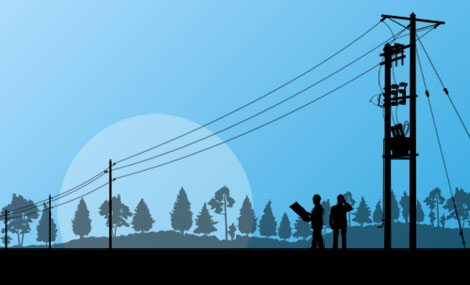
\includegraphics[scale=0.23]{inspection_people}
  \hspace{0.1cm}
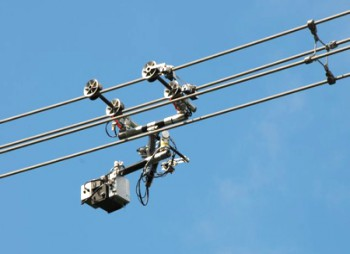
\includegraphics[scale=0.26]{inspection_robot}
  \hspace{0.1cm}
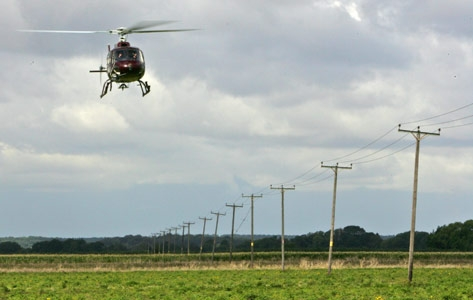
\includegraphics[scale=0.22]{inspection_helicopter}
\end{figure}
\end{frame}

\begin{frame}[t, fragile]{r/MildlyInteresting}
\begin{figure}
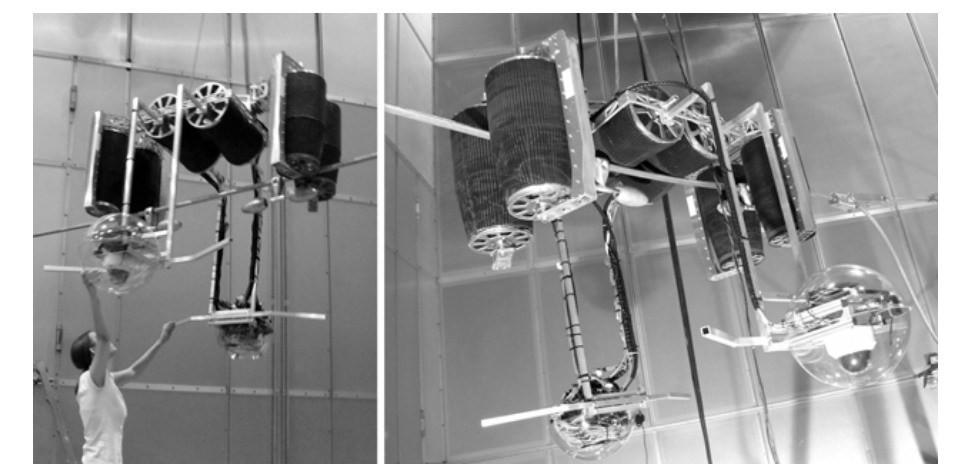
\includegraphics[scale=0.33]{canuimagine}
\end{figure}
\end{frame}

\begin{frame}[t, fragile]{Problem Statement}
Given:
\begin{itemize}
\item Set of images taken from UAV
\item Camera poses (e.g. extracted through any SFM pipeline)
\item 3D model of the scene, lacking power pylons
\item \lbrack Optional\rbrack  Calculated digital elevation model (DEM)
\end{itemize}
The goal is to:
\begin{itemize}
\item Estimate power pylon positions with sub-meter precision
\item Insert pylons into the model
\end{itemize}
\end{frame}

\section{Existing Solutions}

\begin{frame}[t, fragile]{Approaches Overview}
\begin{figure}
\centering
\includegraphics[width=0.8\linewidth]{approaches.png}
\label{fig:line3d_output}
\end{figure}
\end{frame}


\begin{frame}[t, fragile]{Approaches Overview: Photogrammetry + LiDAR}
Gunho Sohn et al. "Automatic Powerline Scene Classification and Reconstruction Using Airborne LiDAR Data", 2012 
\begin{itemize}
\item Split space into voxels 1.5 x 1.5 x 1.5 $\Rightarrow$ line voting, RANSAC
\item Pylon detection: RF classifier
\begin{itemize}
\item Maximum orientation variation (huge for pylons)
\item Orientation parallelism
\end{itemize}
\item Pylon detection: 0.06m for power lines
\end{itemize}
\end{frame}

\begin{frame}[t, fragile]{Approaches Overview: Photogrammetry + LiDAR}
Li et al. "A Model-Driven Approach for 3D Modeling of Pylon from Airborne LiDAR Data", 2015
\begin{itemize}
\item Model-based approach (library of pylon heads)
\item Detection via height variance map and density projection image
\item Position and orientation: contour planes; assume verticality
\item Precision: said to be 0.03m in horizontal plane and 0.99$^\circ $
\end{itemize}
\begin{center}
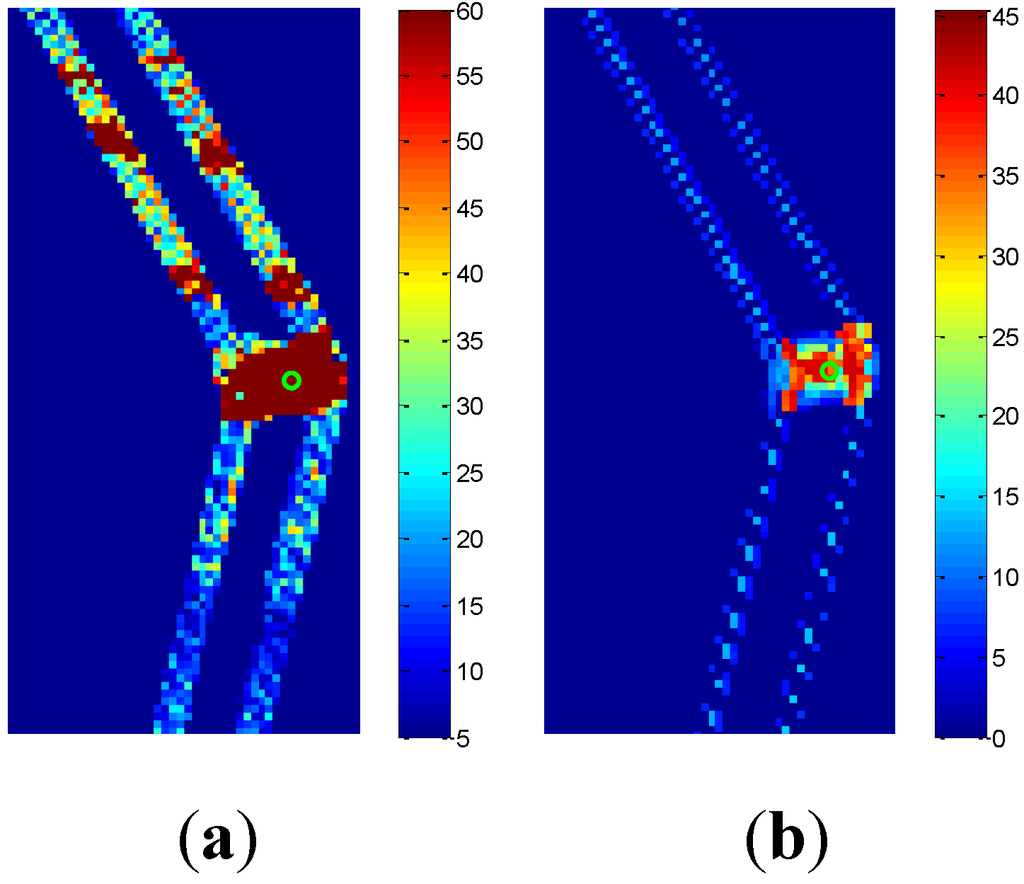
\includegraphics[width=0.3\linewidth]{model_based_lidar1}
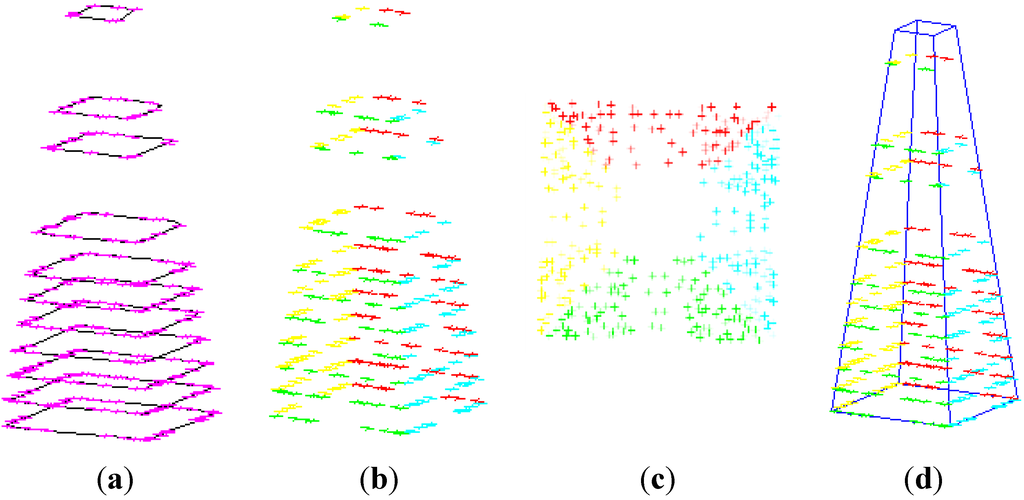
\includegraphics[width=0.5\linewidth]{model_based_lidar3}
\end{center}

\begin{flushright}
\small{$^*$Pictures from original work}
\end{flushright}
\end{frame}

\begin{frame}[t, fragile]{Approaches Overview: Photogrammetry + LiDAR}
 Bo Guo et al. "A Stochastic Geometry Method for Pylon
Reconstruction from Airborne LiDAR Data", 2016
\begin{itemize}
\item Model-based approach (library of pylons)
\item Simulated annealing to match models
\item Precision: said to be 0.37m
\end{itemize}
\end{frame}

\begin{frame}[t, fragile]{Approaches Overview: Pure Photogrammetry}

Disclaimer: SIFT + PMVS perform poorly: wiry structures are thin and textureless $\Rightarrow$ small amount of feature points 

\begin{itemize}
\item [4] M. Hofer, "Line-based 3D Reconstruction of Wiry Objects", 2013.
\item [4'] M. Hofer, "Efficient 3D scene abstraction using line segments", 2016
\item [5] A. Correa, "UAV vision system: Application in electric line following and 3D reconstruction of associated terrain", 2017
\item [6] B. Morarjee, "Using Multiple View Geometry for Transmission Tower Reconstruction", 2016

\item [7] O. Araar, N. Aouf, "Power pylon detection and monocular depth
estimation from inspection UAVs", 2015
\end{itemize}
\end{frame}

\begin{frame}[t, fragile]{Key ideas of [4]}
Line3D is an open source C++ library which reconstructs 3d line segments form the set of images, developed as PhD by Manuel Hofer
\begin{itemize}

\item Supports many SFM frameworks
\item Can be used either standalone or as a library
\item Key ideas: 
\begin{itemize}
\item 2d LSD on each image
\item large set of 3d matching hypotheses (epipolar matching)
\item color histogram similarity
\item collinearity
\end{itemize}
\end{itemize}
Unfortunately, very poor results when wiry object is far and the number of photos is small
\end{frame}

\begin{frame}[t, fragile]{Line3D Timing}
Data taken from [4], time is in minutes
\begin{figure}
\centering
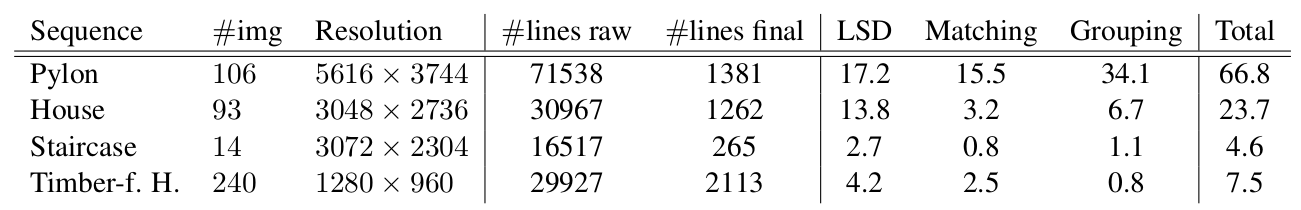
\includegraphics[scale=0.25]{line3dtime}
\end{figure}

[4'] improves runtime significantly (up to 8 times)
\end{frame}


\begin{frame}[t, fragile]{Line3D output sample}

\begin{figure}
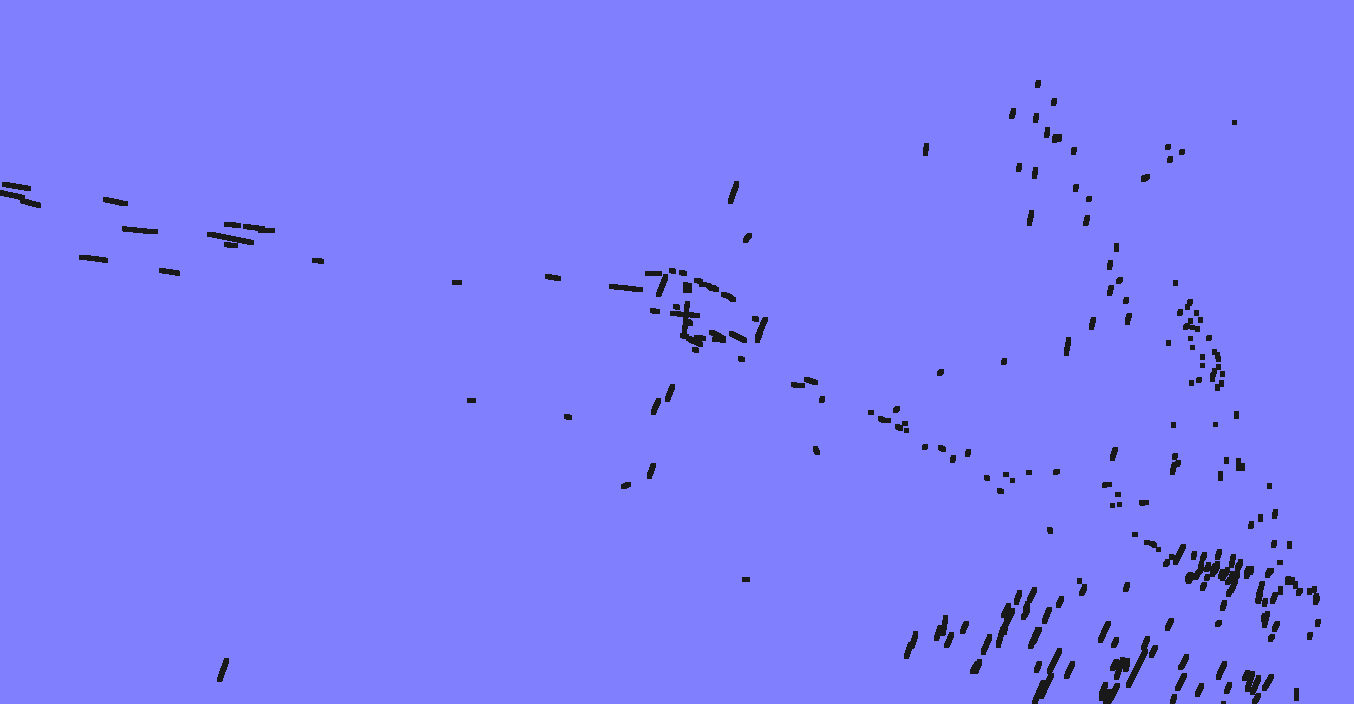
\includegraphics[width=1\linewidth]{line3d_output}
\captionsetup{labelformat=empty}
\caption{Maybe, this can be used...}
\end{figure}
\end{frame}



\begin{frame}[t, fragile]{Key ideas of [5]}
\begin{itemize}
\item [1] Power line detection
\item [2] \textbf{Power towers detection}
\item [3] UAV visual-based navigation
\item [4] \textbf{3D reconstruction of electrical infrastructure}
\end{itemize}

\begin{itemize}
\item Custom line detection algorithm Circle Based Search
\begin{itemize}
\item Said to be faster than Hough/LSD when dealing with long lines
\item Not so precise with short lines; but it is feature in case of wire detection
\end{itemize}
\item Pylon detection through SVM
\begin{itemize}
\item ORB descriptor for features
\item ROI is splitted into cells and for each cell decision is made
\item Time per image (640 x 480) is 25 ms 
\end{itemize}
\end{itemize}
\end{frame}

\begin{frame}[t, fragile]{Key ideas of [6]}
M. Hofer's epigon: uses Line3d

\begin{figure}
\centering
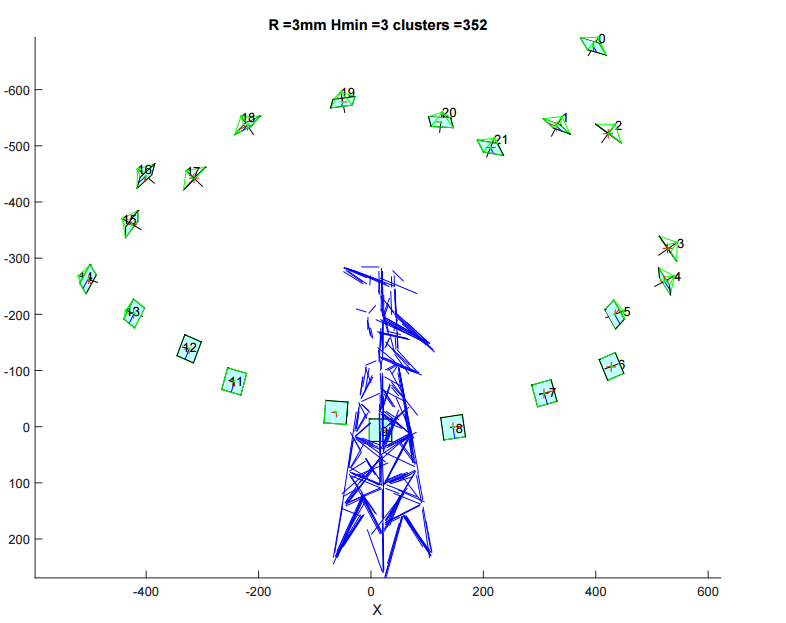
\includegraphics[scale=0.25]{morrarjee}
\captionsetup{labelformat=empty}
\caption{Typical result}
\end{figure}
\end{frame}

\begin{frame}[t, fragile]{Interesting idea of [7]}
\begin{figure}
\centering
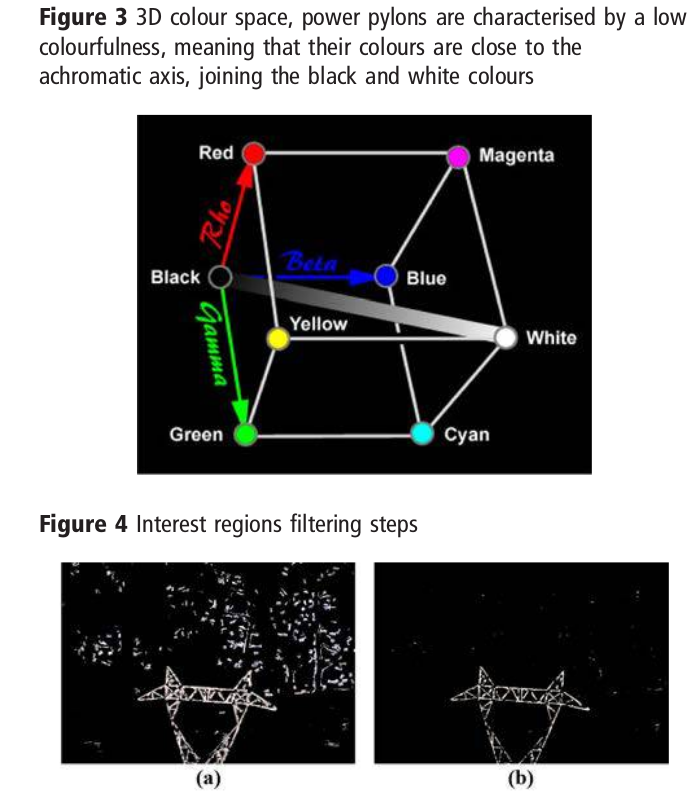
\includegraphics[scale=0.23]{colorful}
\end{figure}
\end{frame}

\section{Suggested Approach}

\begin{frame}[t, fragile]{Overview}
\begin{figure}
\centering
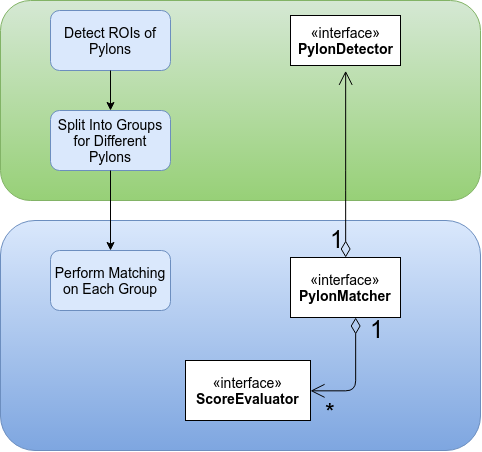
\includegraphics[scale=0.37]{Pipeline}
\captionsetup{labelformat=empty}
\caption[a]{Solution pipeline and key entities}
\end{figure}
\end{frame}

\begin{frame}[t, fragile]{Pylon Detection}
Current simple (yet working in non-urban scenes) strategy:
\begin{itemize}
\item Find power wires
\item Wires intersection $\Rightarrow$ pylon
\item Knowing pylon height and having DEM, evaluate 3d point and project on neighbor images
\end{itemize}
Interestingly, never seen it used anywhere
\begin{itemize}
\item Probably due to inefficiency: $\approx$ 3 seconds per photo (6000x4000)
\item Probably due to problems in urban areas
\end{itemize}
\end{frame}



\begin{frame}[t, fragile]{Feasibility}

\begin{figure}[H!]
\centering
\begin{subfigure}{.5\textwidth}
\centering
\includegraphics[width=1\linewidth]{dirhard}
\caption{Input image (wires are emphasized)}
\end{subfigure}%
\begin{subfigure}{.5\textwidth}
\centering
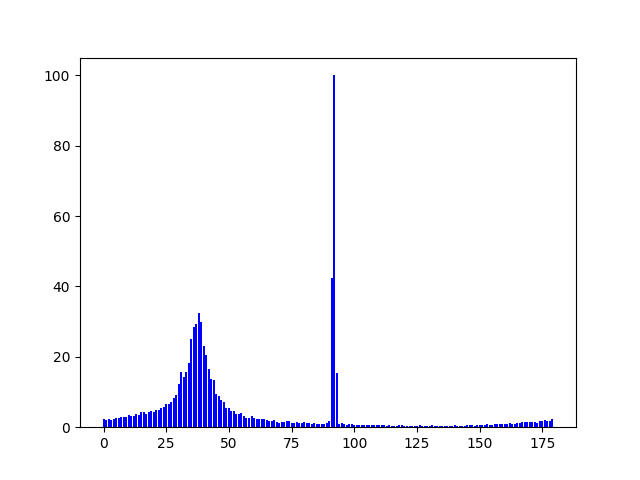
\includegraphics[width=1\linewidth]{dirhisthard}
\caption{Normalized sum of segments square lengths by direction}
\end{subfigure}
\end{figure}
\end{frame}



\begin{frame}[t, fragile]{Pylon Detection}
\begin{figure}
\centering
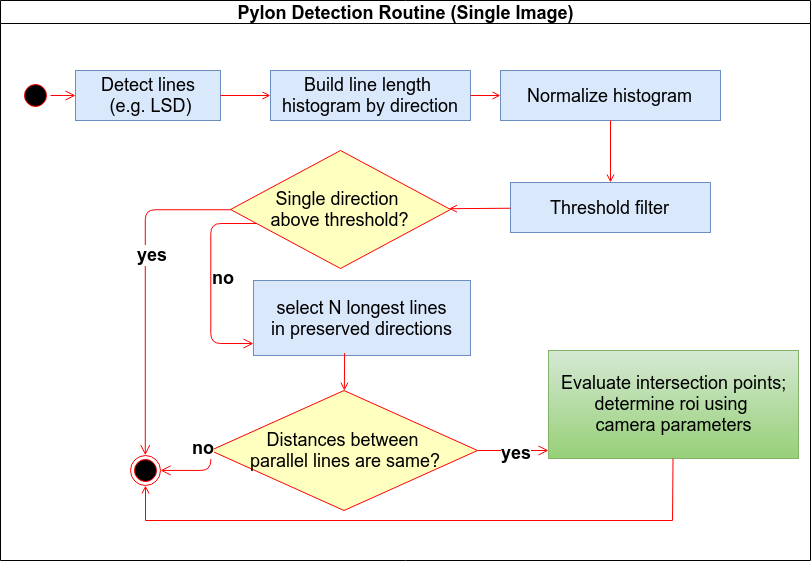
\includegraphics[scale=0.33]{DetectionSimple}
\end{figure}
\end{frame}

\begin{frame}[t, fragile]{Possible Pylon Detection Enhancements}
\begin{itemize}
\item Maybe use CBS algorithm proposed in \lbrack 5\rbrack
\item Use some ML for efficiency and robustness
\begin{itemize} 
\item SVM or neural networks
\end{itemize}
\item Look for many triangles in the seen
\end{itemize}
\end{frame}


\begin{frame}[t, fragile]{Detection Results Example}
\begin{figure}
\centering
\begin{subfigure}{.5\textwidth}
\centering
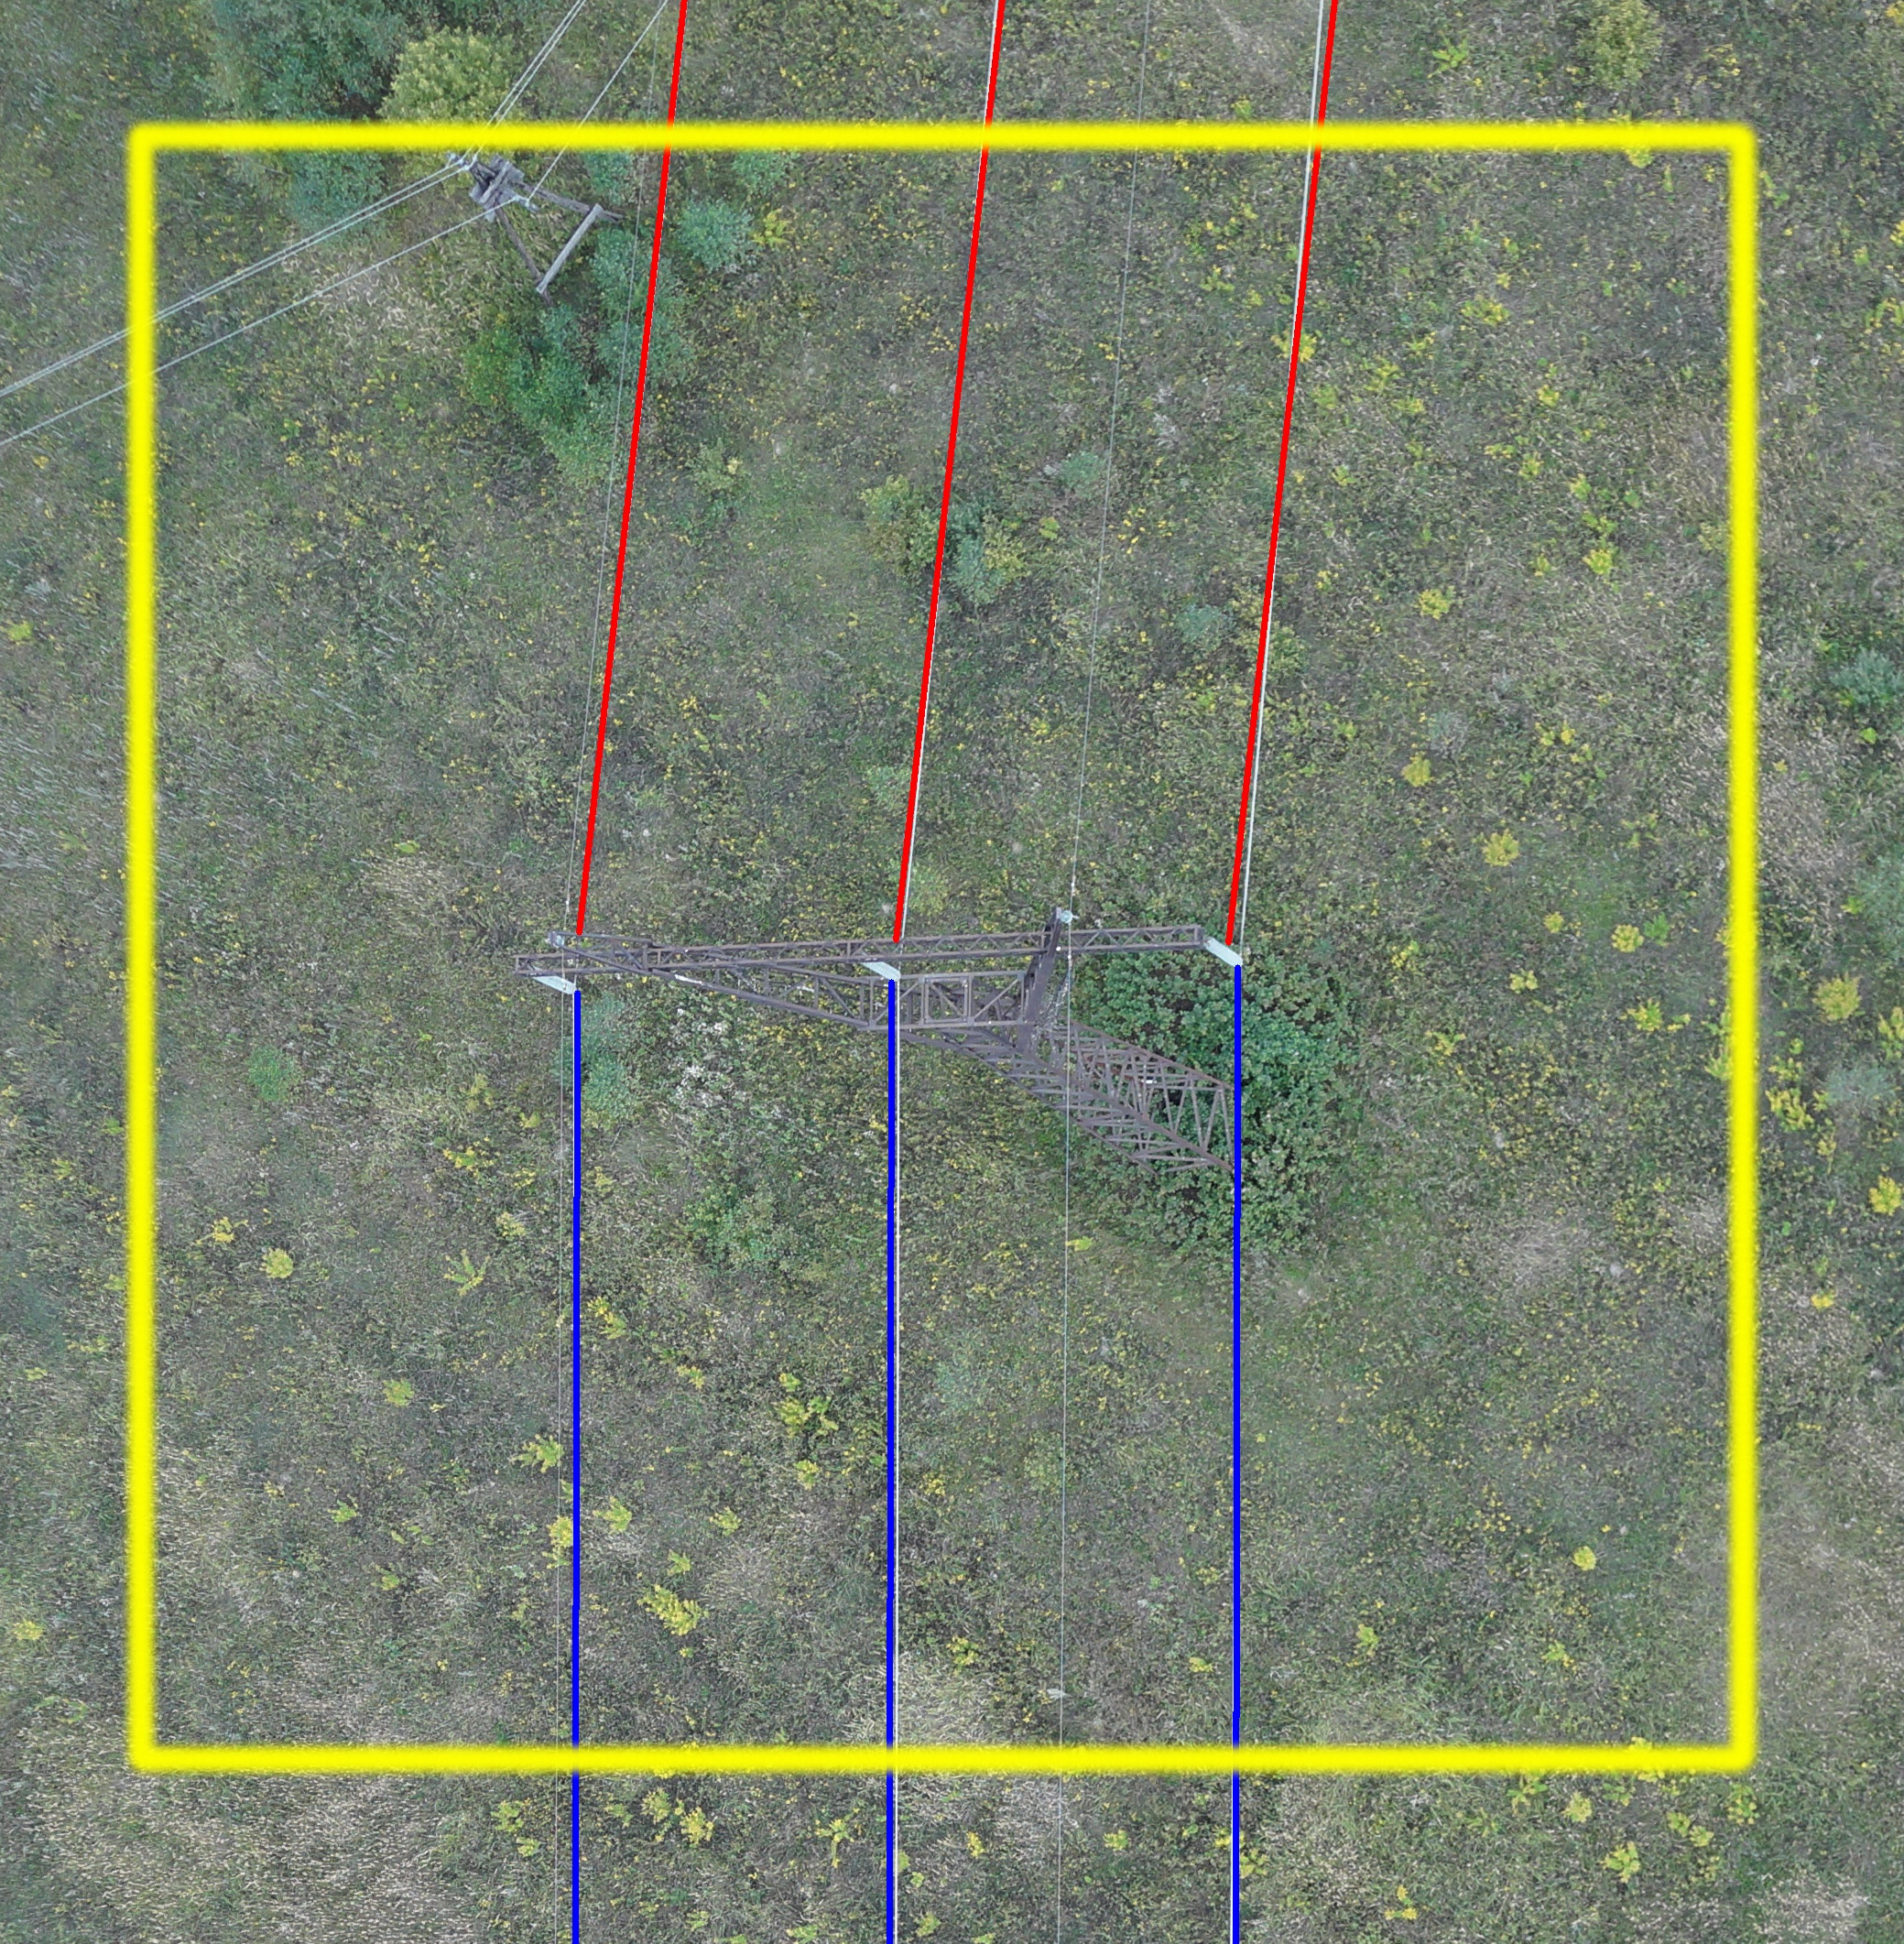
\includegraphics[scale=0.07]{intersection1}
\caption{Detected pylon}
\end{subfigure}%
\begin{subfigure}{.5\textwidth}
\centering
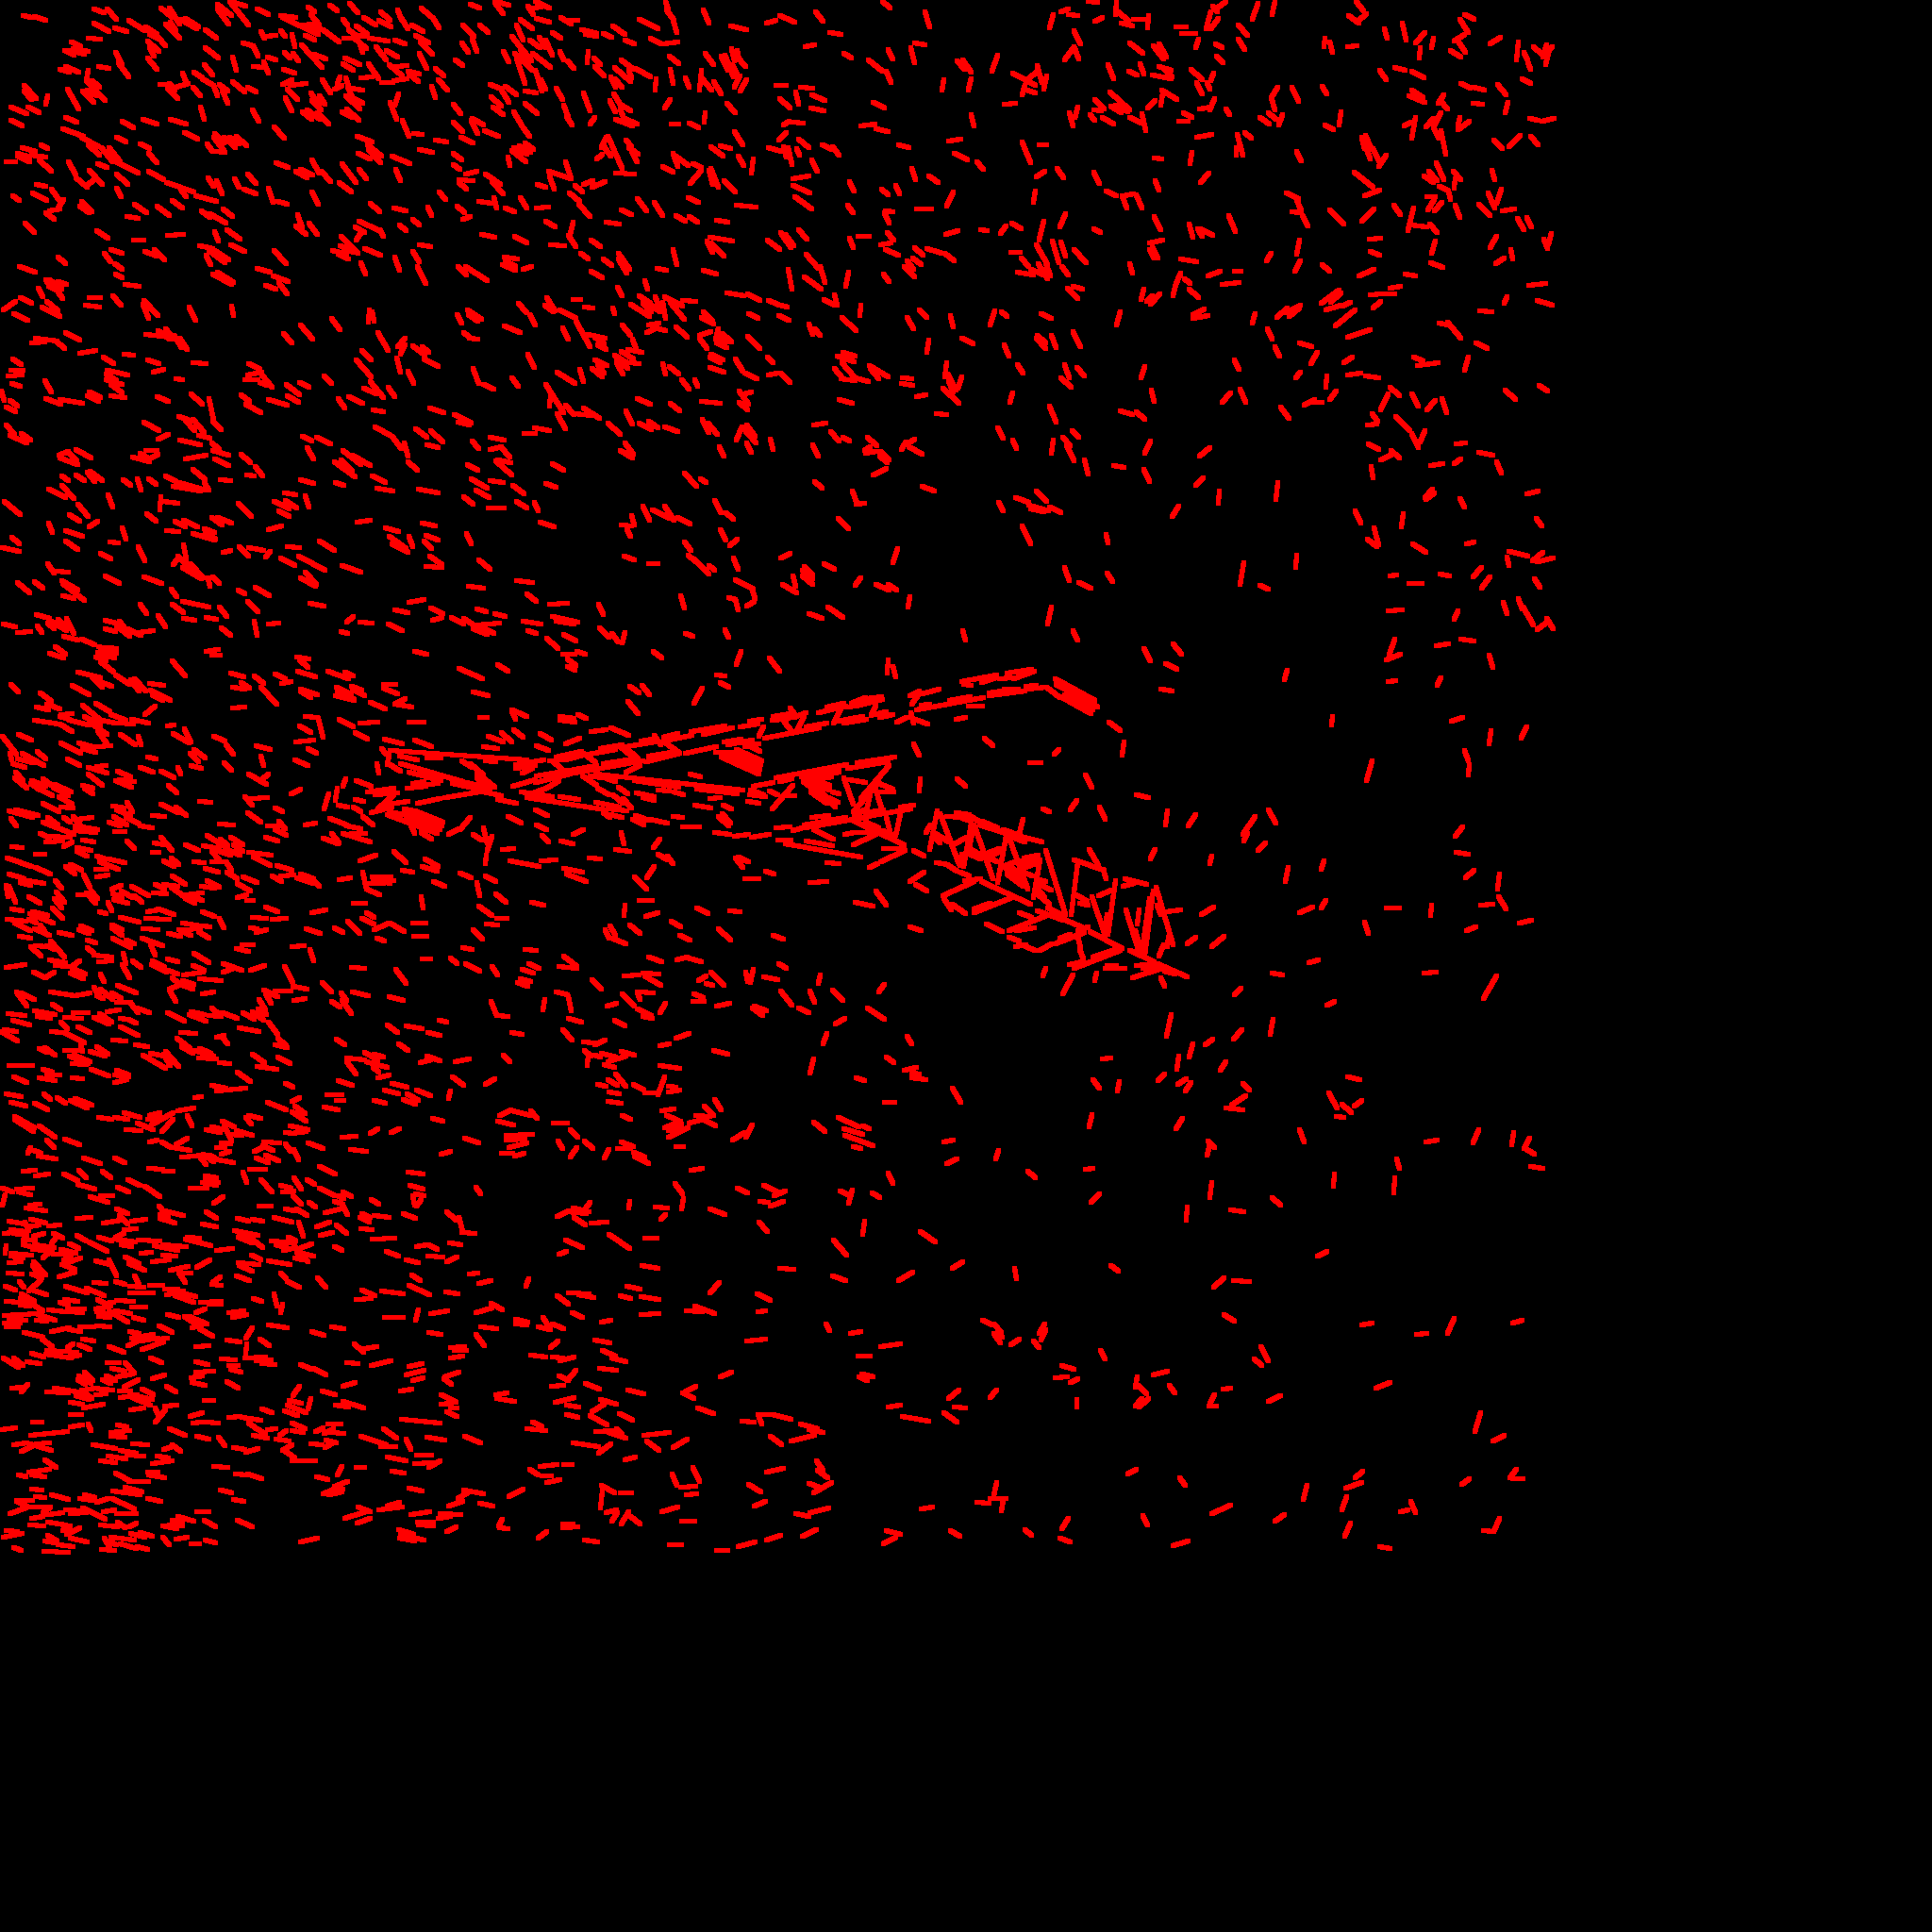
\includegraphics[scale=0.072]{roi}
\caption{Extracted roi lines}
\end{subfigure}
\end{figure}
\end{frame}


\begin{frame}[t, fragile]{Pylon Matching}
\begin{itemize} 
\item Match photos independently
\item Combine results
\end{itemize}

Two matchers are currently implemented: exhaustive and triangle
\begin{itemize} 
\item \textbf{Exhaustive matcher} gets cartesian and angle boundaries as input and naively busts transformations   
\begin{itemize} 
\item Precise, usually works fine if boundaries are set correctly
\item Can be extremely slow
\end{itemize} 
\item \textbf{Triangle matcher} finds triangle holes on the CAD model $\{t_m\}$ and triangles on the image $\{t_i\}$, and for each pair ($t_m, t_i$) tries to find model transformation matrix $M$: $P \cdot V \cdot M(t_m) = t_i$   
\begin{itemize}
\item It's enough to solve $4^{th}$ order polynomial equation for a single triangles pair
\item Produces hypotheses, some are incorrect $\Rightarrow$ need sanity check (scoring, common sense)
\item Generally a lot faster than exhaustive search
\item Sometimes there are too few of image triangles $\Rightarrow$ not a silver bullet
 
\end{itemize}
\end{itemize}

\end{frame}

\begin{frame}[t, fragile]{Model holes and Image Triangles}
\begin{figure}
\centering
\begin{subfigure}{.5\textwidth}
\centering
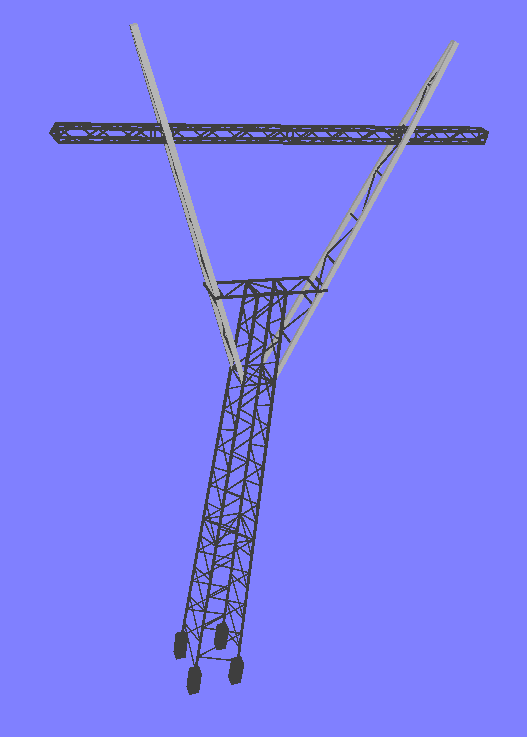
\includegraphics[scale=0.22]{3d_model}
\caption{Original model}
\end{subfigure}%
\begin{subfigure}{.5\textwidth}
\centering
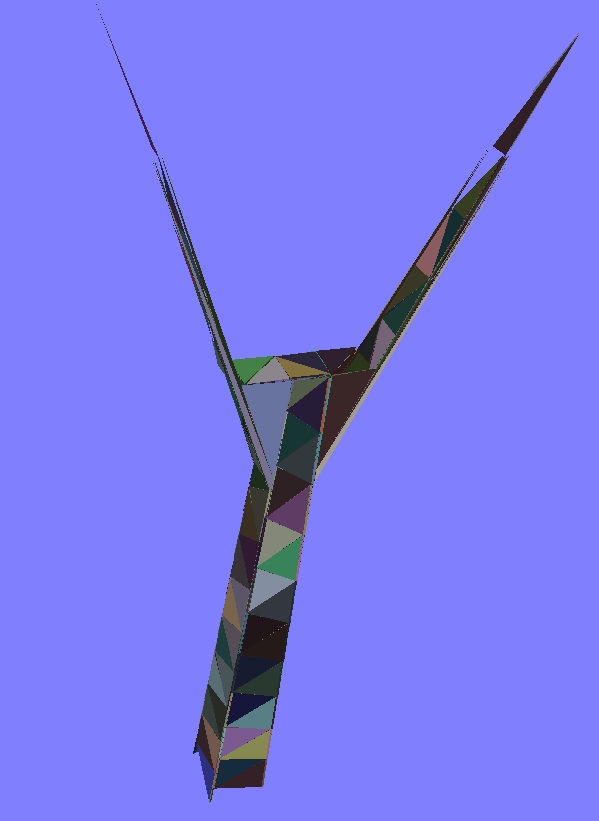
\includegraphics[scale=0.2]{colored_3d_triangles}
\caption{Extracted triangle holes}
\end{subfigure}
\end{figure}
\end{frame}


\begin{frame}[t, fragile]{Pylon Matching}

\begin{figure}
\centering
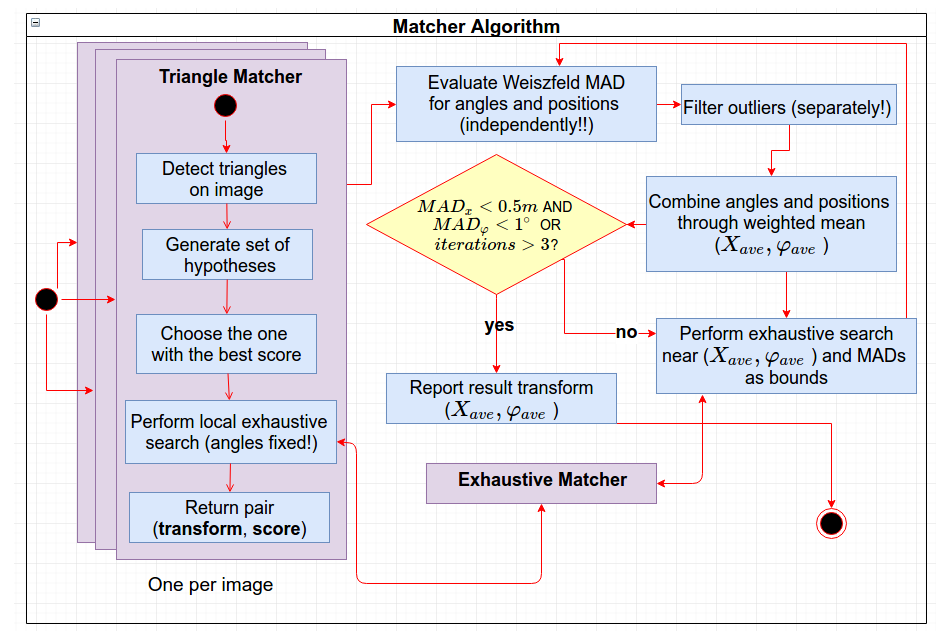
\includegraphics[scale=0.3]{Match}
\end{figure}
 

\end{frame}



\begin{frame}[t, fragile]{Triangle Matching Example}
\vspace{1cm}
\begin{figure}
\centering
\begin{subfigure}{.5\textwidth}
\centering
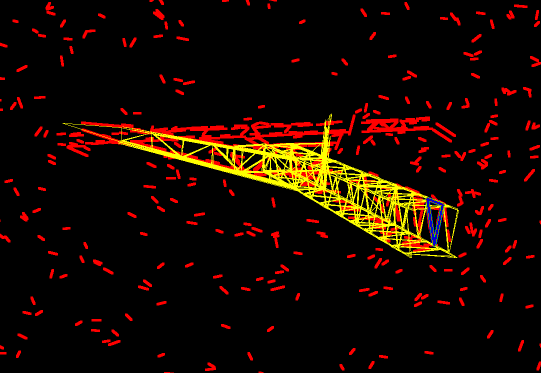
\includegraphics[scale=0.27]{triangle_match}
\caption{Best match}
\end{subfigure}%
\begin{subfigure}{.5\textwidth}
\centering
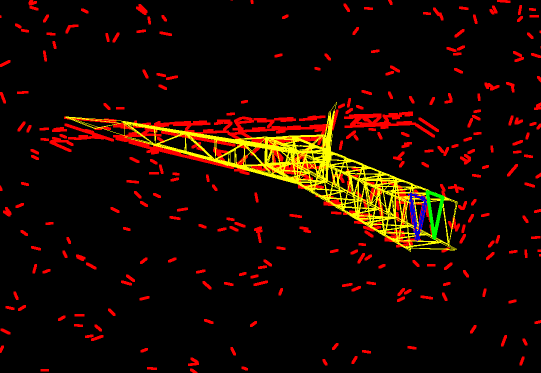
\includegraphics[scale=0.27]{triangle_match_refine}
\caption{After exhaustive refinement}
\end{subfigure}
\end{figure}
\end{frame}





\begin{frame}[t, fragile]{Score Evaluation Approaches}
\begin{itemize}
\item Pixel-counting approach evaluates overlap (in pixels) of rendered model and image segments
\begin{itemize}
\item Can be used simplified solid model
\item Can exploit GPU (currently OpenGL)
\item Efficiency: 600-700 fps on nvidia 840M with solid model, 1000 fps on nvidia GTX Ti 750
\end{itemize}
\item Directions-voting approach evaluates line directions similarity in rendered and reference images
\begin{itemize}
\item Split image into fixed-size cells (e.g. 4x4 pixels)
\item Register image segments directions in each cell (preprocessing)
\item Score is sum of bins in all cells of rendered image which agree with reference image
\item Can exploit GPU (currently CUDA)
\item Efficiency: 100-200 fps better than previous approach
 
\end{itemize}
\end{itemize}
\end{frame}


\begin{frame}[t, fragile]{Score Evaluation}
\begin{figure}
\centering
\begin{subfigure}{.5\textwidth}
\centering
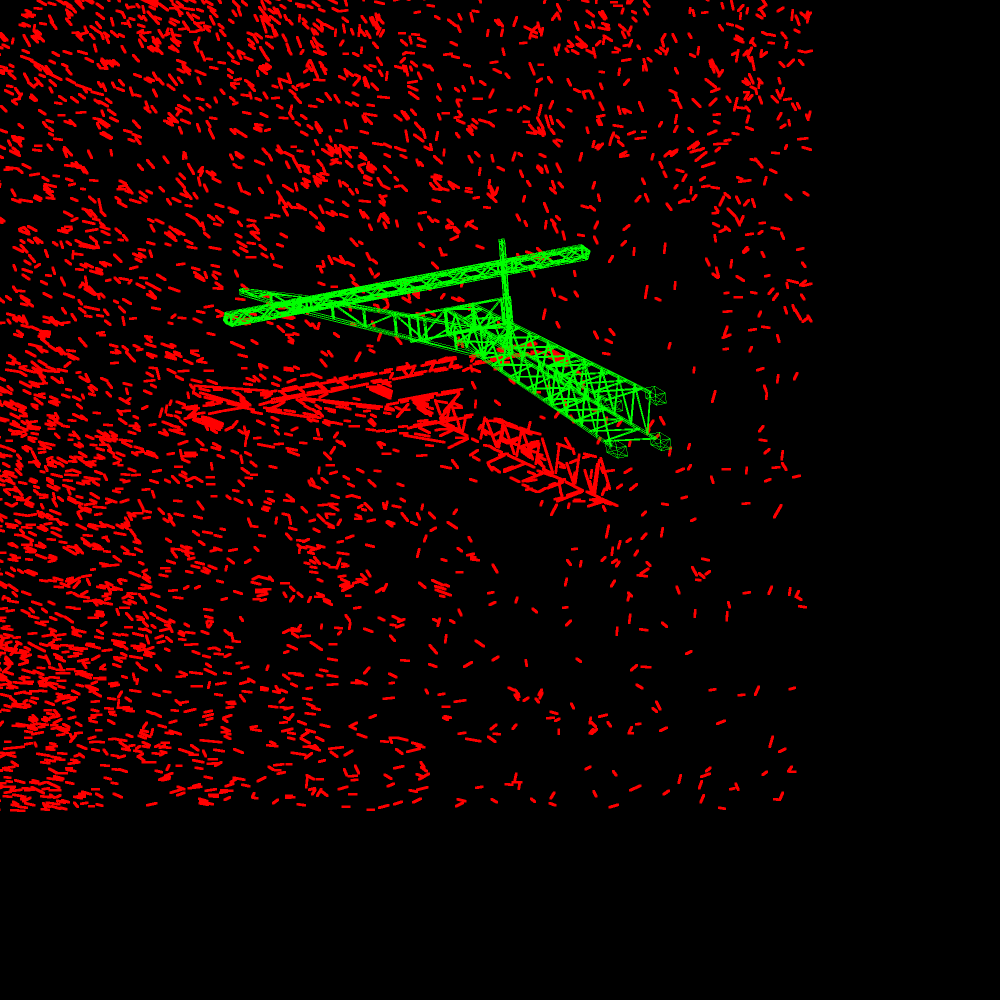
\includegraphics[scale=0.15]{segment_eval}
\caption{Rendered model}
\end{subfigure}%
\begin{subfigure}{.5\textwidth}
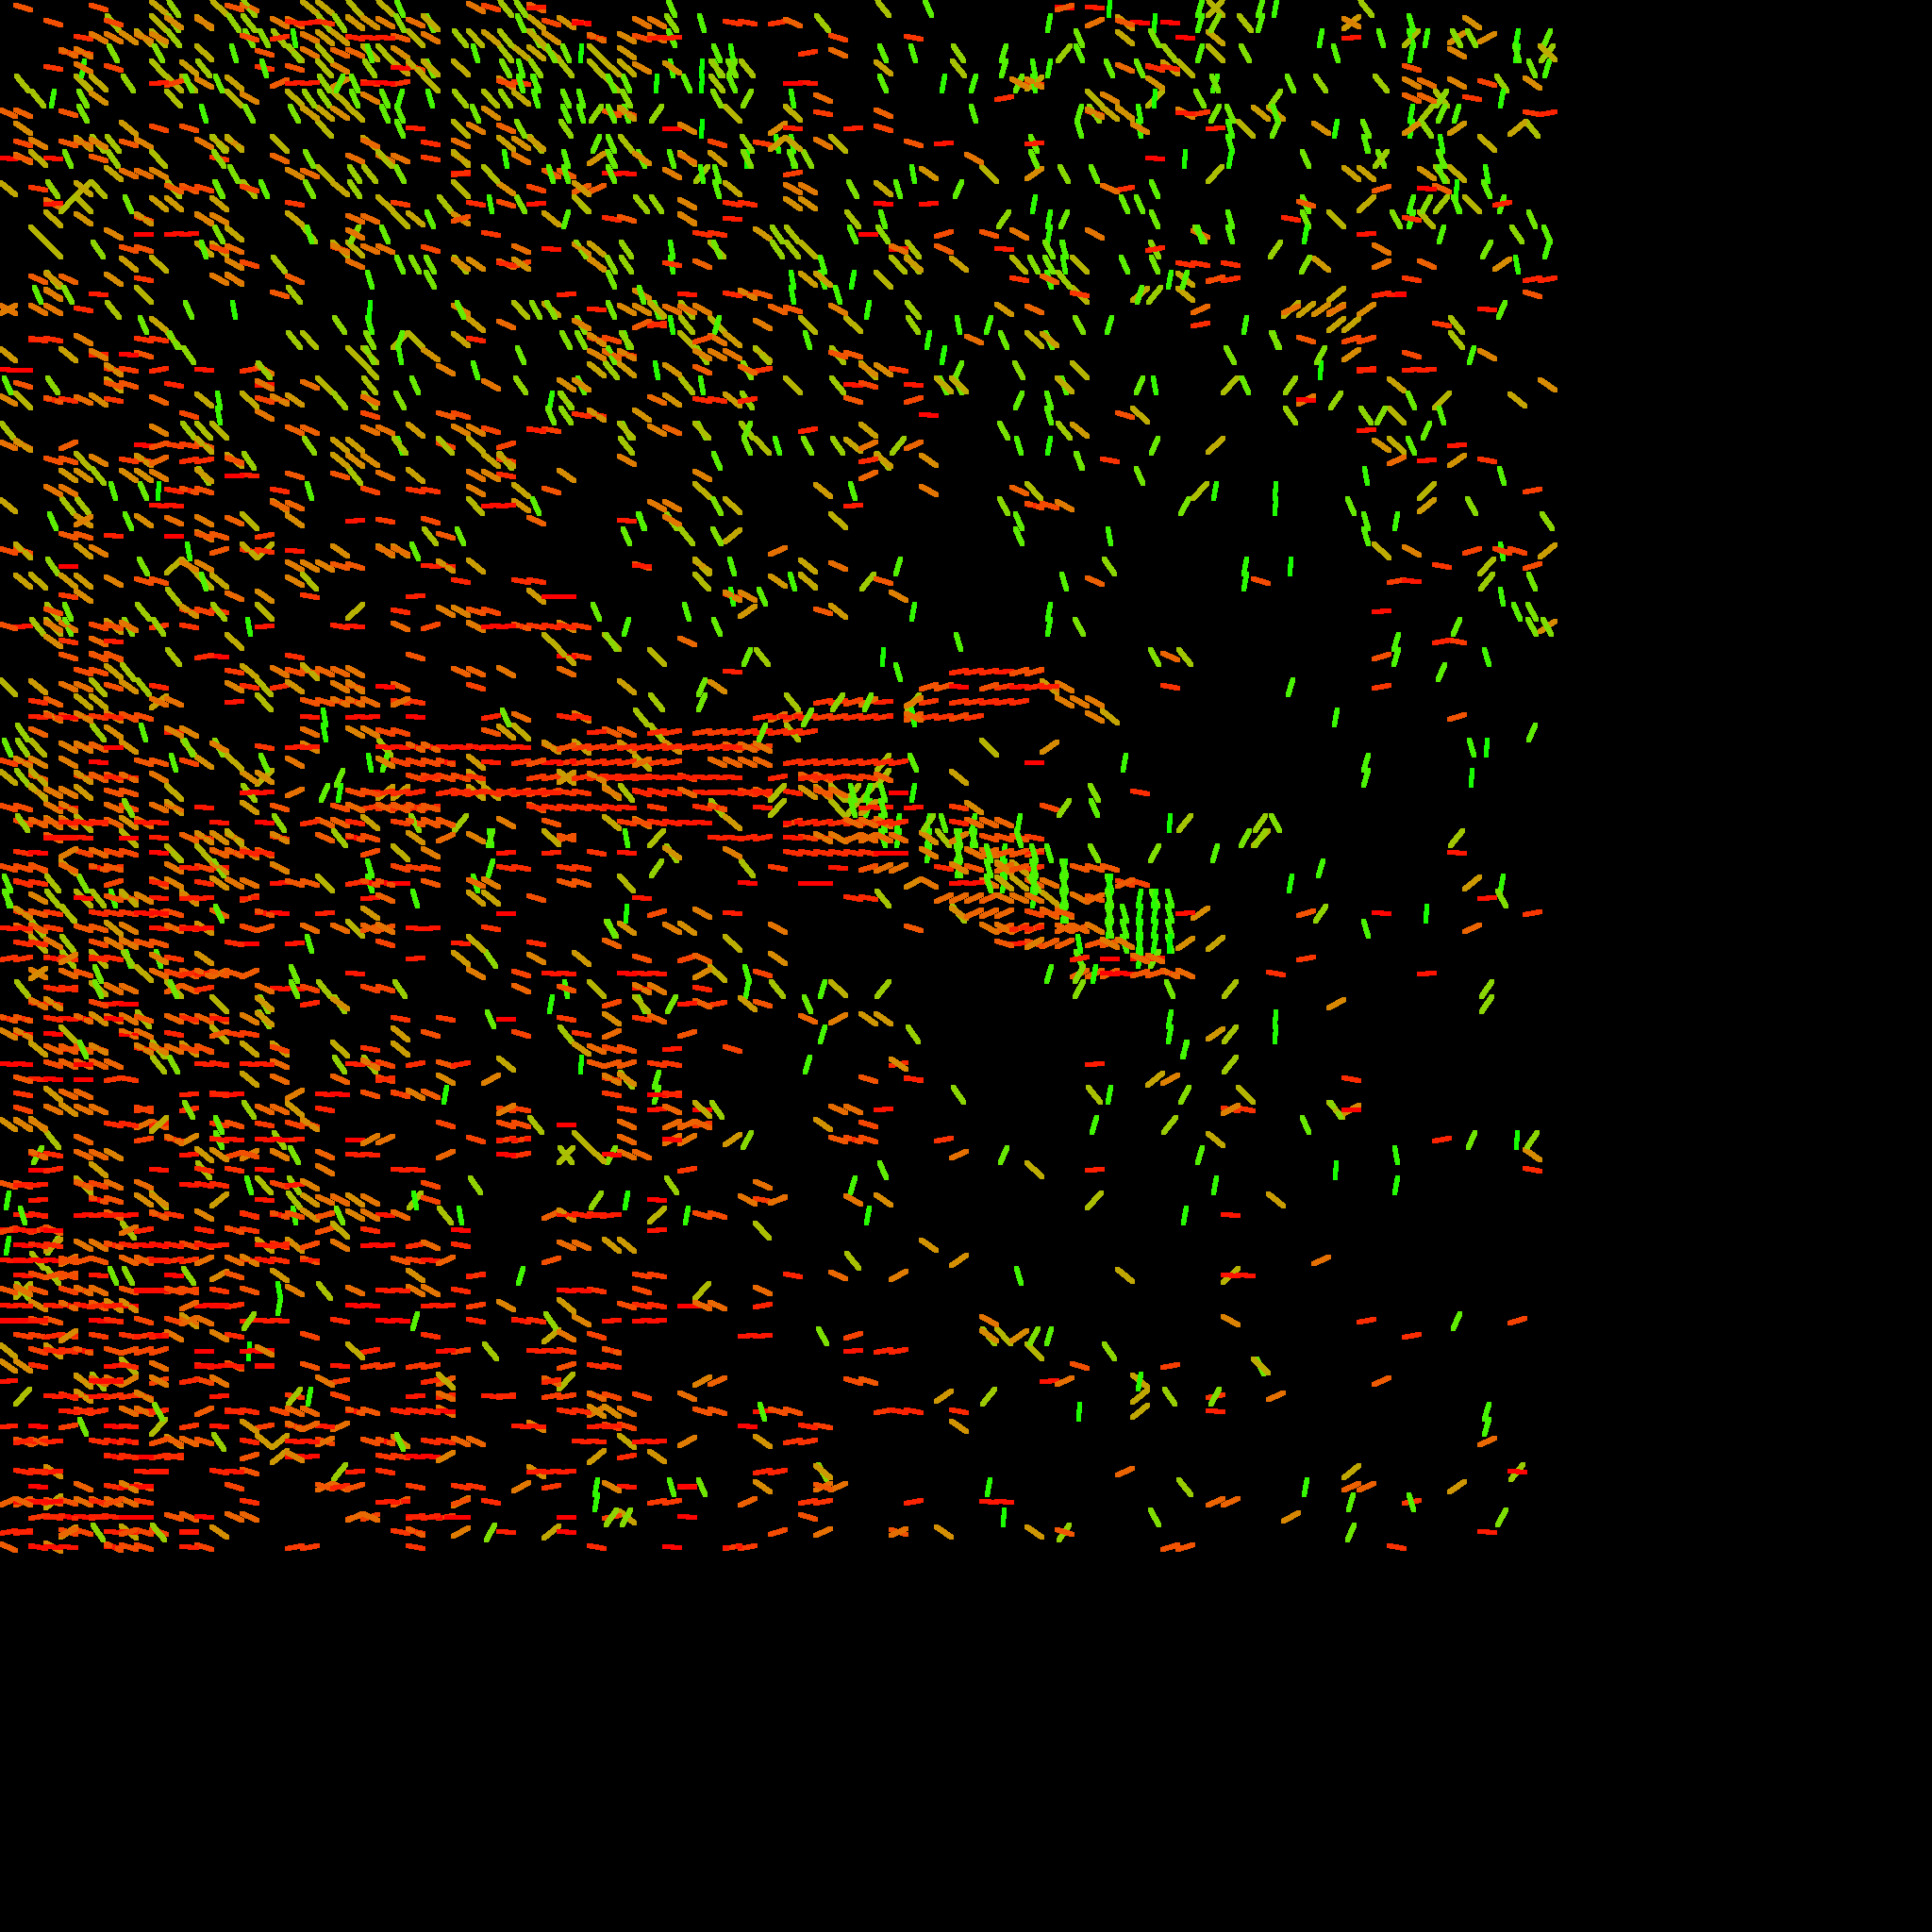
\includegraphics[scale=0.073]{gauss_blur}
\caption{Image cells directions}
\end{subfigure}
\end{figure}
\end{frame}

\begin{frame}[t, fragile]{Solid Model Matching Problems}
\begin{itemize}
\item Noise-sensitive $\Rightarrow$ need to filter non-pylon lines carefully (currently by length)
\begin{itemize}
\item Maybe use graph-cut approach in future with color/orientation/length constraints as seed
\end{itemize}
\item Height estimation (why?)
\begin{itemize}
\item Height is taken from DEM (not good at all!)
\end{itemize}
\end{itemize}
\end{frame}

\begin{frame}[t, fragile]{Directions-Voting Matching}
\begin{itemize}
\item Parallelism: one thread per segment
\item Bresenham's line algorithm for line-grid intersection
\item Score evaluation
\begin{itemize}
\item Evaluate score directly (number of supported reference bins)
\item Convolute reference image with gaussian kernel: i.e. we choose two kernels - 2D kernel for spatial smoothing and 1D kernel for angle smoothing, so that image segment contributes to several bins simultaneously with different weights
\end{itemize}
\end{itemize}
\end{frame}

\begin{frame}[t, fragile]{Results}
\begin{itemize}
\item Currently validated on one test set: 515 photos 6000x4000 with 10 pylons, two of which are of different type then the one which is matched
\item Discrepancy somewhere near 0.4m
\item Using Agisoft Photoscan I have put 3d points, matching them on several images
\item Timings: matching build in debug takes 93 minutes
\begin{itemize}
\item Simple math: Detection took 20 minutes, so average speed is 11.3 minutes per power pylon
\end{itemize}
\end{itemize}
\end{frame}

\begin{frame}[t, fragile]{Results}
\begin{figure}
\centering
\begin{subfigure}{.5\textwidth}
\centering
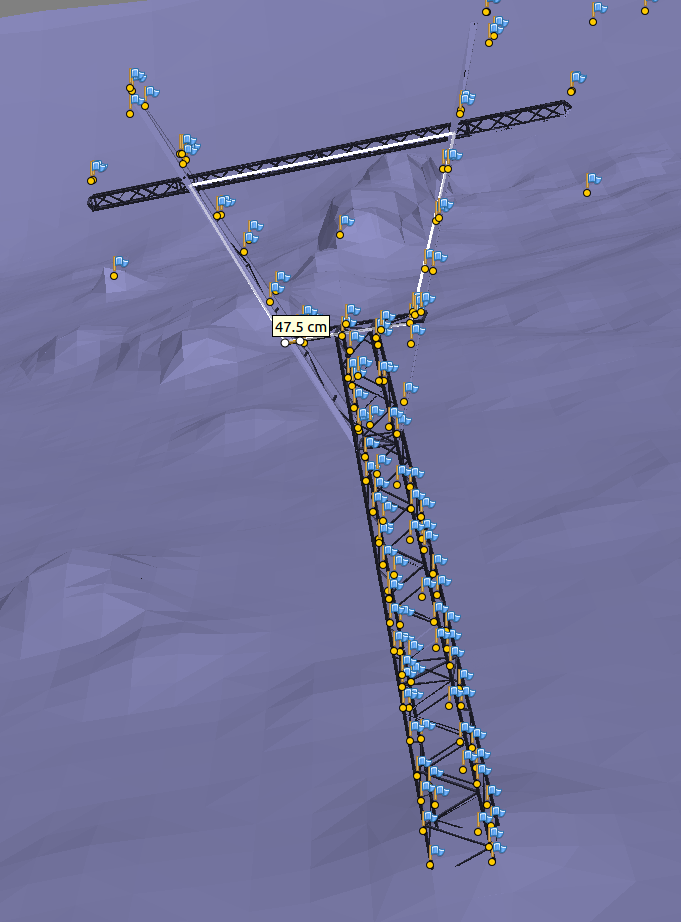
\includegraphics[scale=0.15]{results_cool}
\caption{Inserted 3D model}
\end{subfigure}%
\begin{subfigure}{.5\textwidth}
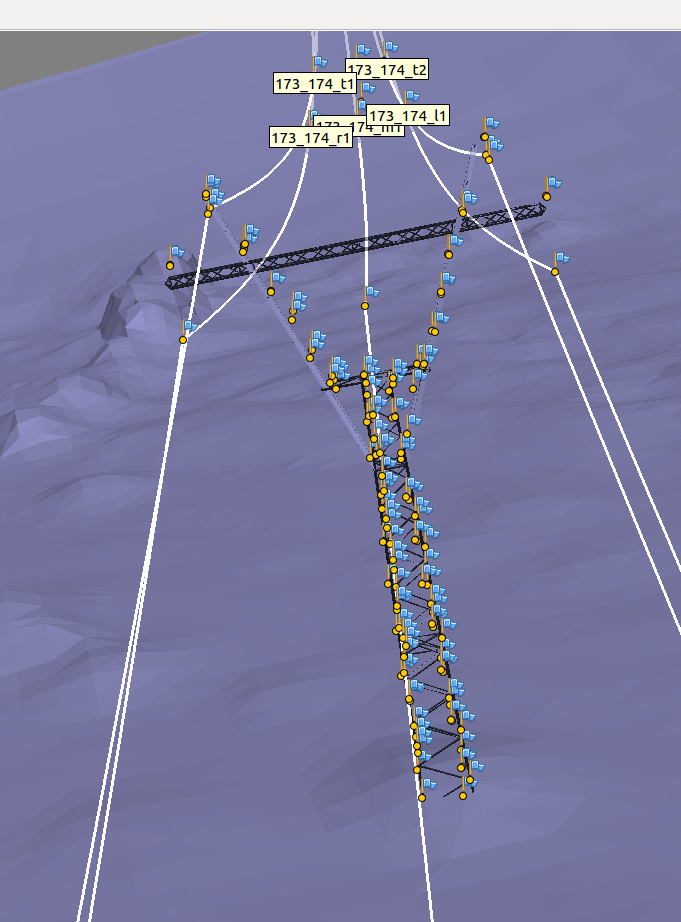
\includegraphics[scale=0.15]{results_cool_wires}
\caption{Wires are added using A. Buslaev's plugin}
\end{subfigure}
\end{figure}
\end{frame}


\begin{frame}[fragile]{Thank You for Your Attention}

\begin{center}
\Huge Q \& A
\end{center}
\end{frame}


\end{document}

